\documentclass[a4paper,10pt,titlepage]{article}

\usepackage[utf8x]{inputenc}
\usepackage[brazil]{babel}
\usepackage{fontenc}
\usepackage{graphicx}
\usepackage{indentfirst}
\usepackage{url}
\usepackage{rotating}

\title{Relatório Técnico-Científico}

\author{{\bf Dhiana Deva Cavalcanti Rocha}
      \\Orientada por José Manoel de Seixas
      \\Laboratório de Processamento de Sinais
      \\Universidade Federal do Rio de Janeiro
      \\Conselho Nacional de Desenvolvimento Científico e Tecnológico
}

\date{\today}

\begin{document}

\maketitle

\tableofcontents

\pagebreak

\listoffigures

\begin{abstract}

Neural Ringer: Filtragem Online Usando Calorimetria de Altas Energias e Redes Neurais

O CERN (Organização Européia para a Investigação Nuclear) é um dos mais importantes centros de pesquisa da atualidade, envolvendo cientistas de diversos países. Com o objetivo de buscar respostas sobre o Universo, a organização é responsável pelo LHC (Grande Colisor de Hádrons), o maior colisor de partículas do mundo. Dentre os experimentos do LHC, o ATLAS é um detector de propósito geral cujo objetivo inclui a procura pelo Bóson de Higgs, partícula que validará o Modelo Padrão de partículas vigente se for observada experimentalmente.

Como o ambiente em questão possui uma alta taxa de eventos e apenas uma parcela muito pequena destes representa informações de interesse físico, ele possui um sistema de filtragem online dividido em três níveis em cascata. O segundo nível, no qual o trabalho está inserido, é dividido em duas etapas consecutivas: extração de características e teste de hipótese.

Uma importante tarefa do sistema de filtragem é selecionar dados de eventos contendo interações de elétrons para uma posterior análise offline, uma vez que estes são fortes indicadores de física de interesse; e eliminar os que são falseados por jatos hadrônicos, que possuem características semelhantes aos elétrons.

O sistema de calorimetria do ATLAS provê dados sobre o perfil da deposição de energia gerado na interação de partículas com seus calorímetros. A partir destes dados é possível estimar o tipo de partícula incidente. O sistema é composto por dois calorímetros: eletromagnético e hadrônico; com quatro e três camadas, respectivamente.

Neste contexto, o Ringer é um pacote de algoritmos desenvolvido pela equipe da UFRJ que visa realizar uma seleção elétron/jato utilizando informações do sistema de calorimetria. Seu módulo de extração de características utiliza uma topologia anelar concêntrica realizada camada a camada para representar de forma compacta perfis de deposição de energia. O módulo de teste de hipóteses realiza a tomada de decisão aplicando técnicas de Redes Neurais a partir do resultado do módulo anterior.

O trabalho realizado envolveu a refatoração do módulo de teste de hipóteses do Ringer. Seu algoritmo de propagação de rede neural foi reescrito de maneira mais simples, ágil, robusta e de acordo com os padrões da colaboração; atingingo uma performance de tempo dezenove vezes melhor que a implementação anterior.

Adicionalmente, foram realizadas análises comparando o comportamento do Ringer e do T2Calo, pacote de referência para a seleção elétron/jato do segundo nível, com dados obtidos experimentalmente sem colisionamento de partículas pelo acelerador, onde Raios Cósmicos constituíram a principal fonte de excitação do sistema de calorimetria e representam eventos que devem ser rejeitados pelo sistema de filtragem. Os resultados obtidos foram fundamentais para comprovar que o trabalho realizado pela equipe mostra-se um potencial candidato para efetiva aplicação durante o experimento, tendo superado a eficiência de rejeição de Raios Cósmicos do T2Calo com 99.56\% frente a 98.21\% do T2Calo.

\end{abstract}

\section{Introdução}

\subsection{CERN - Organização Européia para a Investigação Nuclear}

O CERN é o maior centro de pesquisa de física de partículas do mundo, responsável por um complexo (Figura~\ref{fig:cern_acelerators} de seis aceleradores de partículas com diversas experiências associadas a eles. O CERN também é conhecido por ser onde a WWW (World Wide Web) foi criada, impulsionada pela necessidade de compartilhamento de informações entre os cientistas de diferentes partes do mundo.

\begin{figure}[htbp!]
 \centering
 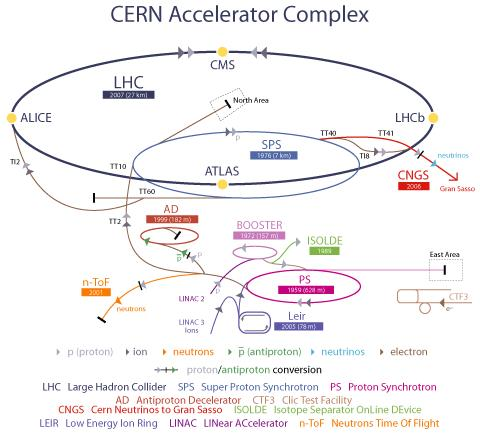
\includegraphics[width=8cm,height=6cm]{Figs/atlas/cern_acelerators.jpeg}
 \caption{Complexo de Aceleradores do CERN}
 \label{fig:cern_acelerators}
\end{figure}

\subsection{LHC - Grande Colisor de Hádrons}

Localizando-se em um túnel de vinte e sete quilômetros de circunferência a cerca de cem metros de profundidade na fronteira entre a França e a Suíça, o LHC \cite{LHC} é o maior e mais poderoso acelerador de partículas existente no mundo, atingindo colisões de valores energéticos nunca antes obtidos em ambientes controlados. Desta maneira, será possível recriar condições semelhantes aos instantes imediatamente posteriores ao fenômeno do Big Bang.

Atualmente o LHC (Figura~\ref{fig:top_view_lhc}) possui sete experimentos: ATLAS, CMS, ALICE, LHCb, TOTEM, LHCf e o mais recentemente aprovado MoEDAL. Os dois primeiros são detectores de propósito geral, que visam investigar uma vasta gama de físicas de interesse. Os restantes possuem propósitos mais específicos como investigação de partículas exóticas, antimatérias e raios cósmicos.

\begin{figure}[htbp!]
 \centering
 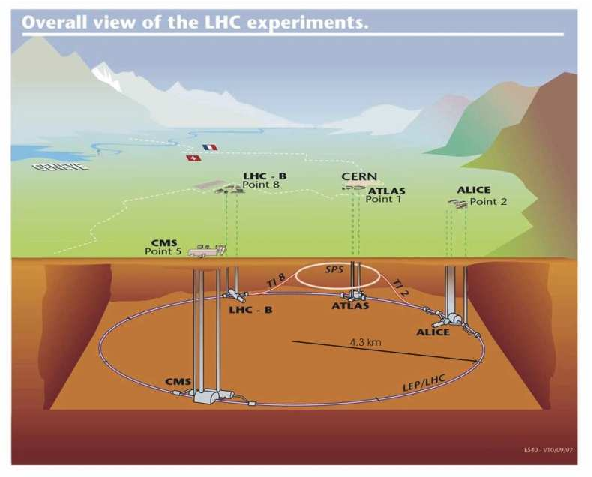
\includegraphics[width=8cm,height=6cm]{Figs/atlas/top_view_lhc.pdf}
 \caption{Vista de cima do LHC}
 \label{fig:top_view_lhc}
\end{figure}

\subsection{O Experimento ATLAS}

Possuindo quarenta e seis metros de comprimento e vinte e cinco metros de largura, o ATLAS \cite{ATLAS} é o maior dos detetores do LHC. Seu objetivo inclui a procura pelo Bóson de Higgs, partícula que validará o Modelo Padrão de partículas vigente se for observada experimentalmente; outras dimensões e a matéria escura.

O ATLAS foi construído de acordo com um formato cilíndrico sendo subdividido em áreas de barril e tampa. Para representar espacialmente o detetor são utilizadas as coordenadas $\eta$ e $\phi$ que indicam, respectivamente, a direção da projeção das partículas e a rotação.

\begin{figure}[htbp!]
 \centering
 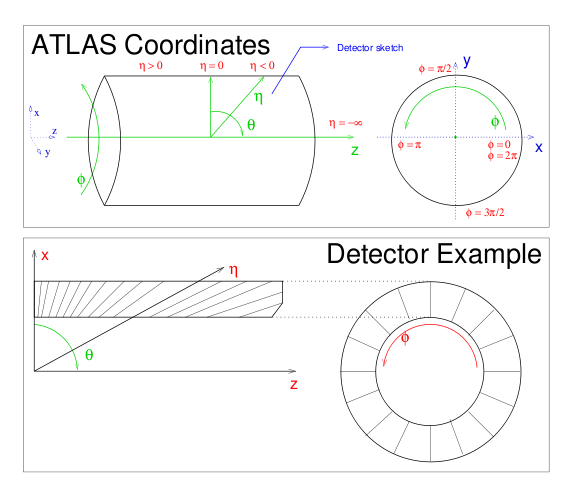
\includegraphics[width=8cm,height=6cm]{Figs/atlas/atlas_coords.png}
 \caption{Sistema de coordenadas do ATLAS}
 \label{fig:atlas_coords}
\end{figure}

O detector possui diferentes módulos que atuam na observação de variados aspectos dos produtos das colisões (Figura~\ref{fig:atlas_detector}). Um importante módulo é o sistema de calorimetria, responsável pela medição de energia das partículas incidentes. Este sistema é composto pelos calorímetros eletromagnético e hadrônico, somando ao todo sete camadas com diferentes granularidades.

\begin{figure}[htbp!]
 \centering
 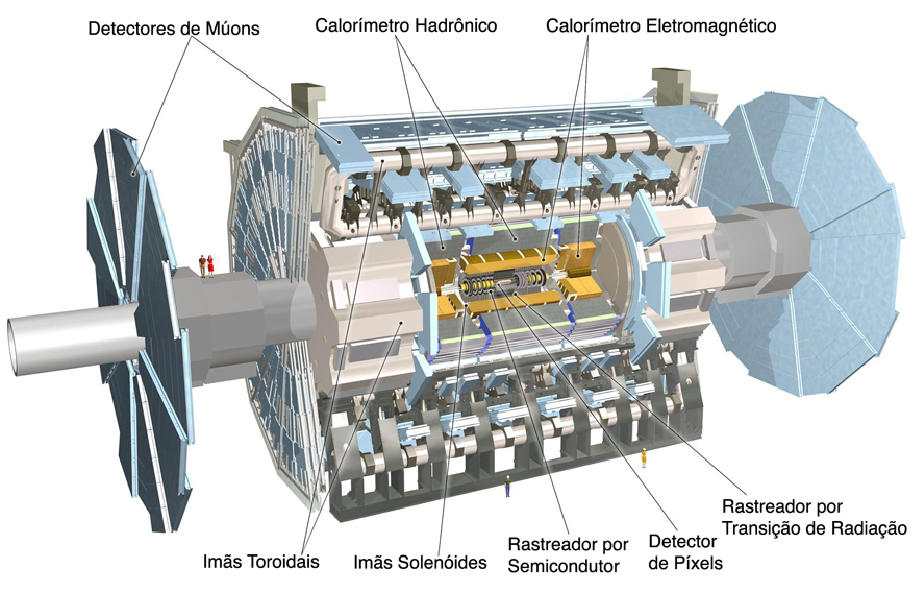
\includegraphics[width=8cm,height=6cm]{Figs/atlas/atlas_detector.pdf}
 \caption{O detector ATLAS e seus módulos}
 \label{fig:atlas_detector}
\end{figure}

A partir das informações do sistema de calorimetria é possível estimar o tipo de partícula incidente, uma vez que cada tipo interage com as sete camadas de maneira distinta (Figura~\ref{fig:decay_chart}).

\begin{figure}[htbp!]
 \centering
 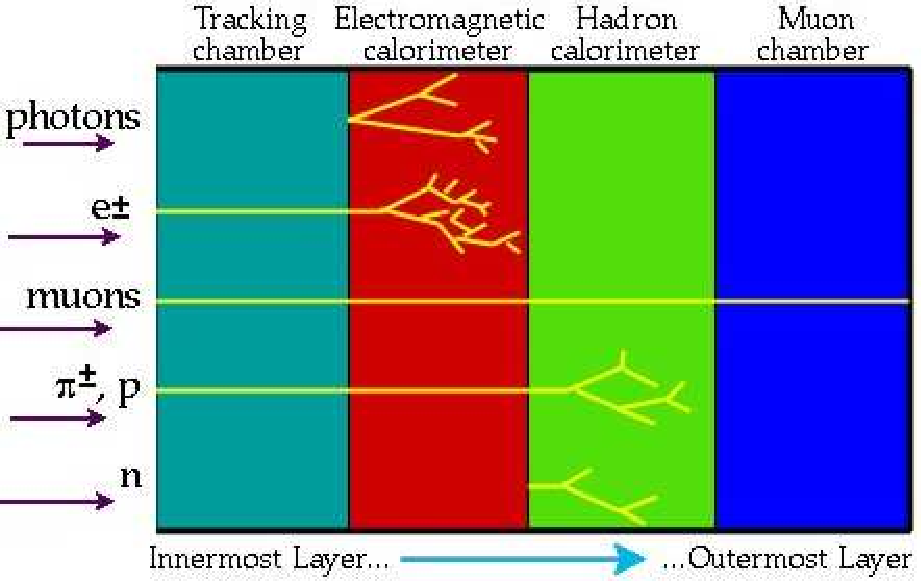
\includegraphics[width=8cm,height=6cm]{Figs/atlas/decay_chart.pdf}
 \caption{Decaímento de partículas nos detectores do ATLAS}
 \label{fig:decay_chart}
\end{figure}

\subsection{Sistema de Filtragem do ATLAS}

O volume de dados gerado pelo detector a cada colisão é enorme e apenas uma parcela muito pequena destes dados de fato representa informações relevantes. Desta maneira, o ATLAS possui um sistema de filtragem online dividido em três níveis em cascata.

\begin{figure}[htbp!]
 \centering
 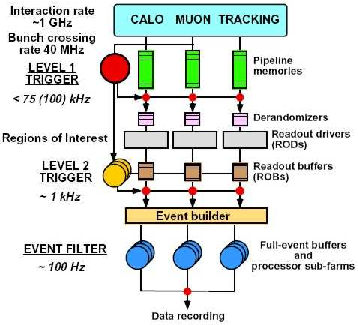
\includegraphics[width=8cm,height=6cm]{Figs/atlas/block_diagram_trigger.pdf}
 \caption{O sistema de filtragem do ATLAS}
 \label{fig:block_diagram_trigger}
\end{figure}

O primeiro nível é responsável pela seleção inicial de regiões de interesse físico atuando a partir de informações dos detectores com granularidade reduzida. Sua implementação é em hardware, de maneira que o tempo de latência seja o mais baixo possível.

Já o segundo nível é implementado em software e utiliza a plena granularidade dos detectores para refinar as informações das regiões selecionadas pelo nível antecedente e assim eliminar eventos com informações irrelevantes, reduzindo a taxa de eventos a serem processados pelo terceiro nível, que por sua vez analisa todos os dados gerados em cada evento e não somente as regiões selecionadas pelo primeiro nível.

Após a filtragem online, os dados são armazenados em disco e disponibilizados para futuras análises pelo sistema de filtragem offline, o qual atua em ambiente sem requisitos mínimos de tempo permitindo análises avançadas com algoritmos mais complexos.

\subsection{Ringer}

O Ringer é um pacote de algoritmos que atua no segundo nível de filtragem do ATLAS utilizando o sistema de calorimetria para a discriminação elétron/jato. Ele está dividido em dois módulos executados em sequência: extração de características e teste de hipótese. O primeiro visa representar de maneira compacta o perfil do chuveiro gerado nas interações das partículas com as diferentes camadas dos calorímetros. Já o segundo, utiliza as informações geradas pelo módulo antecedente para realizar a aprovação ou rejeição do evento.

No módulo de extração de características, primeiramente é encontrada a célula de maior nível energético em cada camada e a partir delas são formados anéis concênticos (Figura~\ref{fig:rings}). Ao final do processo, as células pertencentes ao mesmo anel são somadas. Considerando-se as sete camadas, produz-se um total de 100 somas em anéis. Esta estratégia reduz a dimensão do evento sem comprometer a interpretação física do mesmo.

\begin{figure}[htbp!]
 \centering
 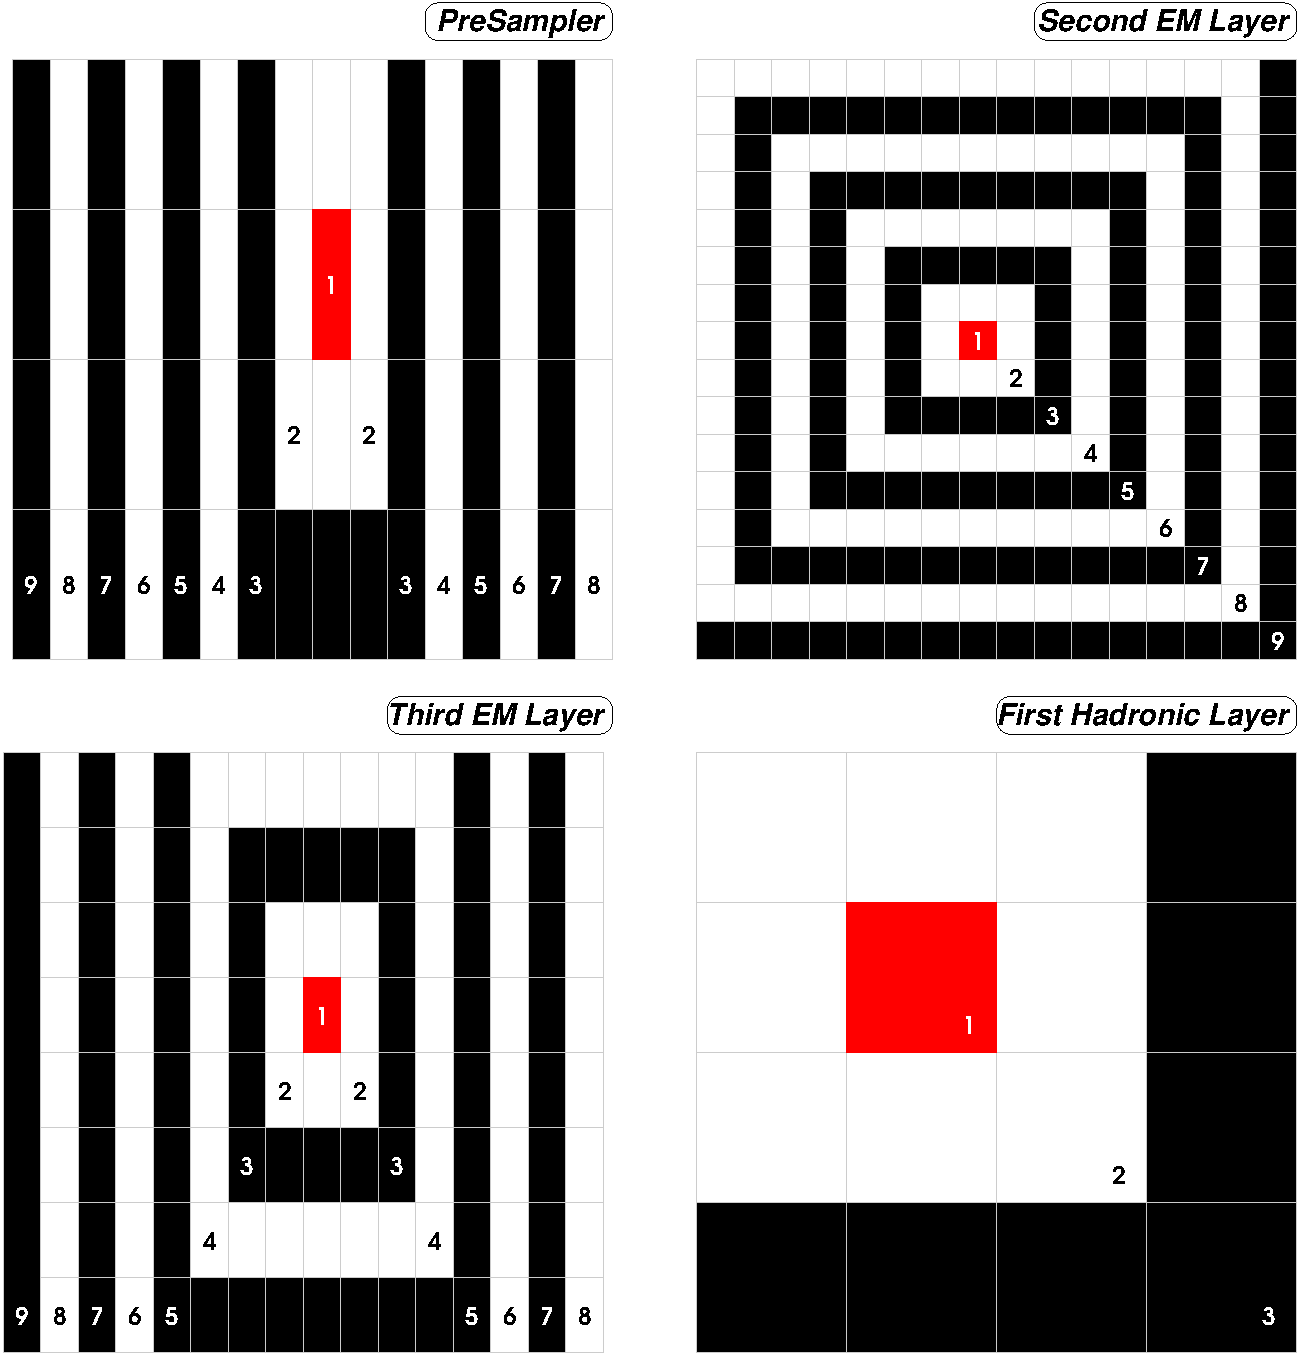
\includegraphics[width=8cm,height=6cm]{Figs/atlas/rings.pdf}
 \caption{Topologia anelar do Ringer}
 \label{fig:rings}
\end{figure}

Os anéis produzidos alimentam o módulo de teste de hipótese, que utiliza redes neurais artificias para a tomada de decisão, permitindo ganhos de eficiência de detecção quando comparados à mecanismos lineares de decisão, como o EgammaHypo, algoritmo de seleção elétron/jato de referência na colaboração.

\section{Tecnologias Utilizadas}

\subsection{Framework Athena}

O framework Athena é um conjunto de pacotes de algoritmos utilizados na filtragem de alto nível do ATLAS. Ele de provê também suporte à uma simulação offline do funcionamento do detector. Sua estrutura é altamente orientada a objetos de maneira a facilitar o entendimento das diversas relações entre os algoritmos e ferramentas.

Os algoritmos do Athena estão subdivididos em três etapas: Inicialização, Execução e Finalização. Dados podem ser compartilhados entre os algoritmos através de uma área de memória temporária - o StoreGate.

\subsection{Framework ROOT}

O framework ROOT é utilizado pela colaboração para a análise de dados gerados pelo experimento. O mesmo possui nativamente um interpretador C++, além de possibilitar acesso através de módulos de extensão Python e Ruby - PyROOT e RubyROOT, respectivamente.

\subsection{Python}

Por ser uma linguagem de alto nível, interpretada, orientada a objetos e com sintaxe facilitada, o Python, ao longo do trabalho realizado, foi a interface mais utilizada para a análise de dados usando o PyROOT. Além disto, a linguagem é padrão para configuração dos algoritmos do framework Athena e desta maneira foi utilizada também em sua utilização.

\subsection{C++}

O desenvolvimento de algoritmos no Athena é realizado utilizando o C++, uma linguagem de programação compilada, fortemente tipada, de nível médio, orientada a objetos e, atendendo os requisitos das aplicações, de alto desempenho. Esta linguagem é de uso bastante popular, desde estudantes até mesmo grandes empresas como Microsoft e Google a utilizam para a implementação de seus softwares.

\subsection{Matlab}

A ferramenta Matlab foi utilizada para a análise de dados e simulação de rede neural por utilizar uma linguagem interpretada de alto nível dirigida para computação técnica, sendo portanto de rápida e eficiente utilização. Gráficos e cálculos numéricos são obtidos de maneira muito mais fácil do que ao utilizar linguagens de programação como C++ ou python.

\section{Metodologia}

Por se tratar de uma colaboração internacional, os códigos foram desenvolvidos utilizando vocabulário técnico em inglês. Também nesta linguagem, foi redigida uma documentação através da ferramenta de escrita colaborativa padrão do CERN - TWiki de maneira a proporcionar à comunidade científica um fácil acesso às informações sobre o pacote Ringer.

Além disto, vale ressaltar que os códigos desenvolvidos para o Athena foram implementados de maneira a gastar o menor tempo e custo computacional possível. Já os scripts de análise de dados foram desenvolvidos priorizando a melhor representação das informações que podem ser extraídas dos dados, além de um desenvolvimento ágil.

Desta maneira os scripts de análises de dados foram desenvolvidos inicialmente em Matlab, pelo sua fácil e rápida obtenção de resultados. No entanto, para disponibilizar as análises para a colaboração, as mesmas foram reproduzidas em ambiente PyROOT. Vale ressaltar que, apesar de ser possível realizar análises interativamente com Matlab e PyROOT, as análises foram realizadas com o desenvolvimento de scripts altamente configuráveis de maneira a possibilitar o reaproveitamento dos mesmos durante a realização do trabalho e até mesmo para futuras análises.

\section{Relatório de Atividades}

\subsection{Refatoração do Pacote TrigMultiVarHypo}

A aluna foi responsável pela refatoração do pacote TrigMultiVarHypo, o módulo de teste de hipótese do pacote Ringer.

O TrigMultiVarHypo está dividido em três etapas:

\begin{itemize}
 \item Inicialização

Executada uma única vez no começo de uma rodada de funcionamento do detector, esta etapa realiza a leitura dos parâmetros configurados em Python de maneira a preparar a rede neural pela qual as somas em anéis serão propagadas a cada evento que for processado pelo módulo de extração de características.

 \item Execução

Esta etapa é responsável por:

 \subitem Aprovar o evento caso este comportamento esteja especificado na configuração da rodada; 
 \subitem Caso contrário, obter as somas em anéis que o módulo de extração de características disponibilizou no StoreGate;
 \subitem Caso os dados obtidos forem compatíveis com a rede configurada, propagá-los pela rede neural;
 \subitem Realizar um corte linear em energia (opcional) e na saída da rede neural de maneira a aprovar ou rejeitar o evento.

 \item Finalização

Executada ao final de uma rodada de funcionamento do detector, esta etapa é responsável pela liberação da memória que fora alocada pelo algoritmo na inicialização.

\end{itemize}

\subsubsection{Implementação Antiga}

Visando possibilitar flexibilidade em relação à topologia da rede neural e funções de ativação de seus neurônios, a implementação antiga possuía uma complexa estrutura orientada a objetos, como pode ser observado na Figura~\ref{fig:old_tmvh}.

\begin{figure}[htbp!]
 \centering
 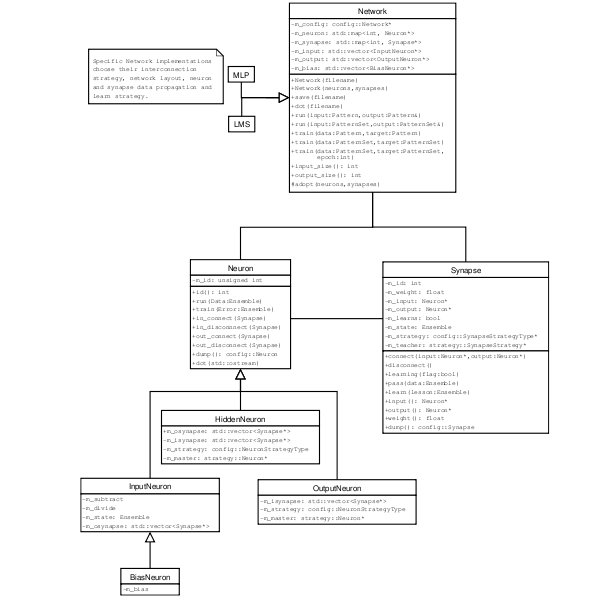
\includegraphics[width=8cm,height=6cm]{Figs/tmvh_refactoring/old_tmvh.jpeg}
 \caption{Diagrama UML da antiga implementação do TrigMultiVarHypo}
 \label{fig:old_tmvh}
\end{figure}

Vale ressaltar que a configuração dos parâmetros da Rede Neural estava sendo realizada através de parâmetros dispostos em formato XML, uma linguagem de marcação desenvolvida com o objetivo de armazenar dados de uma maneira simplificada.

Este conjunto de fatores implicava em um alto custo de uso de memória e de tempo de processamento.

\subsubsection{Nova Implementação}

De maneira a atender os tipos de Redes Neurais treinadas pela equipe, a nova implementação do pacote provê suporte a uma propagação de redes Feed Forward com variável números de camadas, variável número de nós em cada camada e aplica tangente hiperbólica como função de ativação em todos os nós.

Foi criada uma simples estrutura orientada a objeto de maneira a prover os seguintes benefícios:

\begin{itemize}
 \item Configuração em Python:
   \subitem Tornou a configuração do pacote mais acessível e de acordo com os padrões da colaboração.
   \subitem Os parâmetros da rede neural são obtidos através de listas em Python que são então transformadas em matrizes C++.
 \item Código simples:
   \subitem Foi criada uma classe C++ com construtor, destrutor e um método de propagação.
   \subitem A propagação é realizada através de simples multiplicações de matrizes.
 \item Melhor performance de tempo e menor custo de memória:
   \subitem Multiplicações de matrizes utilizam poucos recursos e têm rápida execução.
   \subitem Alocações (maior consumo de tempo/memória) são realizadas somente na inicialização do sistema.
   \subitem São utilizados iteradores de acordo com a especificação mais ágil (ou seja, ++i ao invés de i++).
 \item Robustez garantida:
   \subitem São tratados casos de má alocação, abortando a cadeia de processamento na inicialização e impedindo acesso a endereços inválidos de memória na finalização.
   \subitem Os parâmetros da rede neural são validados.
   \subitem É verificada a compatibilidade dos anéis gerados com a rede construída.
\end{itemize}

\subsubsection{Validação da Saída}

Para validar a correta implementação da nova propagação de rede neural foi criada uma versão de debug do algoritmo. Desta maneira, os anéis gerados e a respectiva saída da rede neural são escritos em um arquivos texto no formato csv (comma-separated-values - valores separados por vírgula), que são facilmente lidos pelo Matlab.

Foi criado um script Matlab possibilitando ler dois arquivos csv (um referente à implementação antiga e outro à nova) e a partir deles plotar um scatter plot dos valores obtidos nos dois métodos além de apontar valores como desvio padrão, skewness, valores máximos e média da diferença.

A Figura~\ref{fig:new_tmvh_splot} nos mostra que foi mantida a consistência da saída da rede neural, indicando que a nova implementação foi realizada corretamente.

\begin{figure}[htbp!]
 \centering
 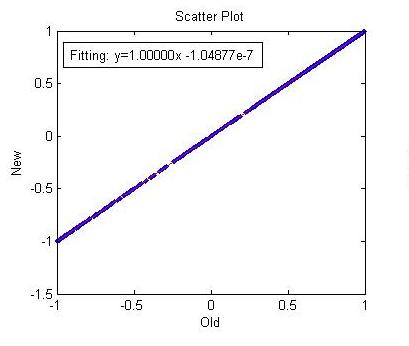
\includegraphics[width=8cm,height=6cm]{Figs/tmvh_refactoring/new_tmvh_splot.jpeg}
 \caption{Scater plot da saída da rede neural utilizando as implementações antiga e nova do TrigMultiVarHypo}
 \label{fig:new_tmvh_splot}
\end{figure}


\subsubsection{Ferramentas de Apoio}

Além do script desenvolvido para realizar a validação da saída da rede neural, foi também desenvolvido um script para exportação dos parâmetros de uma rede neural estruturada no Matlab para a sintaxe python esperada pelo pacote no Athena, uma vez que os estudos feitos pela equipe para treinamento de redes neurais estão sendo realizados utilizando o Matlab.

\subsubsection{Performance de Tempo e Memória}

Através da tabela abaixo podemos concluir que a refatoração do algoritmo foi responsável por um tempo de execução dezenove vezes mais rápido.

\begin{table}[htbp!]
 \centering

 \title{\textbf{Tempo de Execução (ms)}}

 \begin{tabular}{cc}
  \hline Antiga Implementação & $ 0.2047 \pm 0.0558 $\\
  \hline Nova Implementação & $ 0.0104 \pm 0.0016 $\\
 \end{tabular}
\end{table}

Somado a isto, também pode ser observado através da figura~\ref{fig:new_tmvh_maloc} que o algoritmo não apresenta vazamento de memória.

\begin{figure}[htbp!]
 \centering
 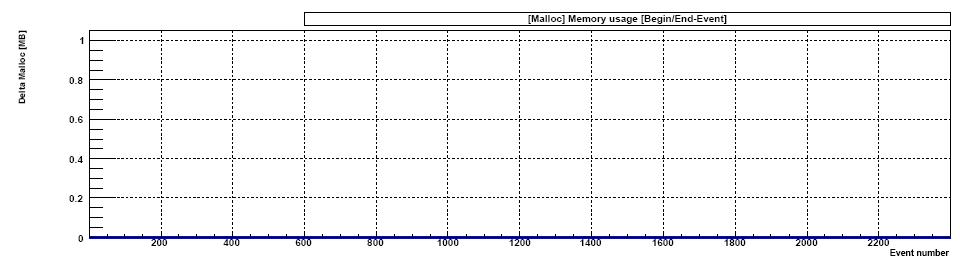
\includegraphics[width=10cm,height=4cm]{Figs/tmvh_refactoring/new_tmvh_maloc.jpeg}
 \caption{Gráfico de alocação de memória na nova implementação do TrigMultiVarHypo}
 \label{fig:new_tmvh_maloc}
\end{figure}

\subsection{Análises com Dados Experimentais}

Foi realizada a aquisição e análise de dados experimentais obtidos em rodadas de funcionamento do ATLAS sem eventos de colisão. Neste contexto, a principal fonte de excitação do sistema de calorimetria são raios cósmicos, que são formados por partículas que viajam em velocidades próximas à da luz sendo compostos majoritariamente por prótons. Conforme os Raios Cósmicos penetram na atmosfera, eles sofrem interações com moléculas de gases atmosféricos e, desta maneira, dão origem a novas partículas (Figura~\ref{fig:rc_sky}). 

\begin{figure}[htbp!]
 \centering
 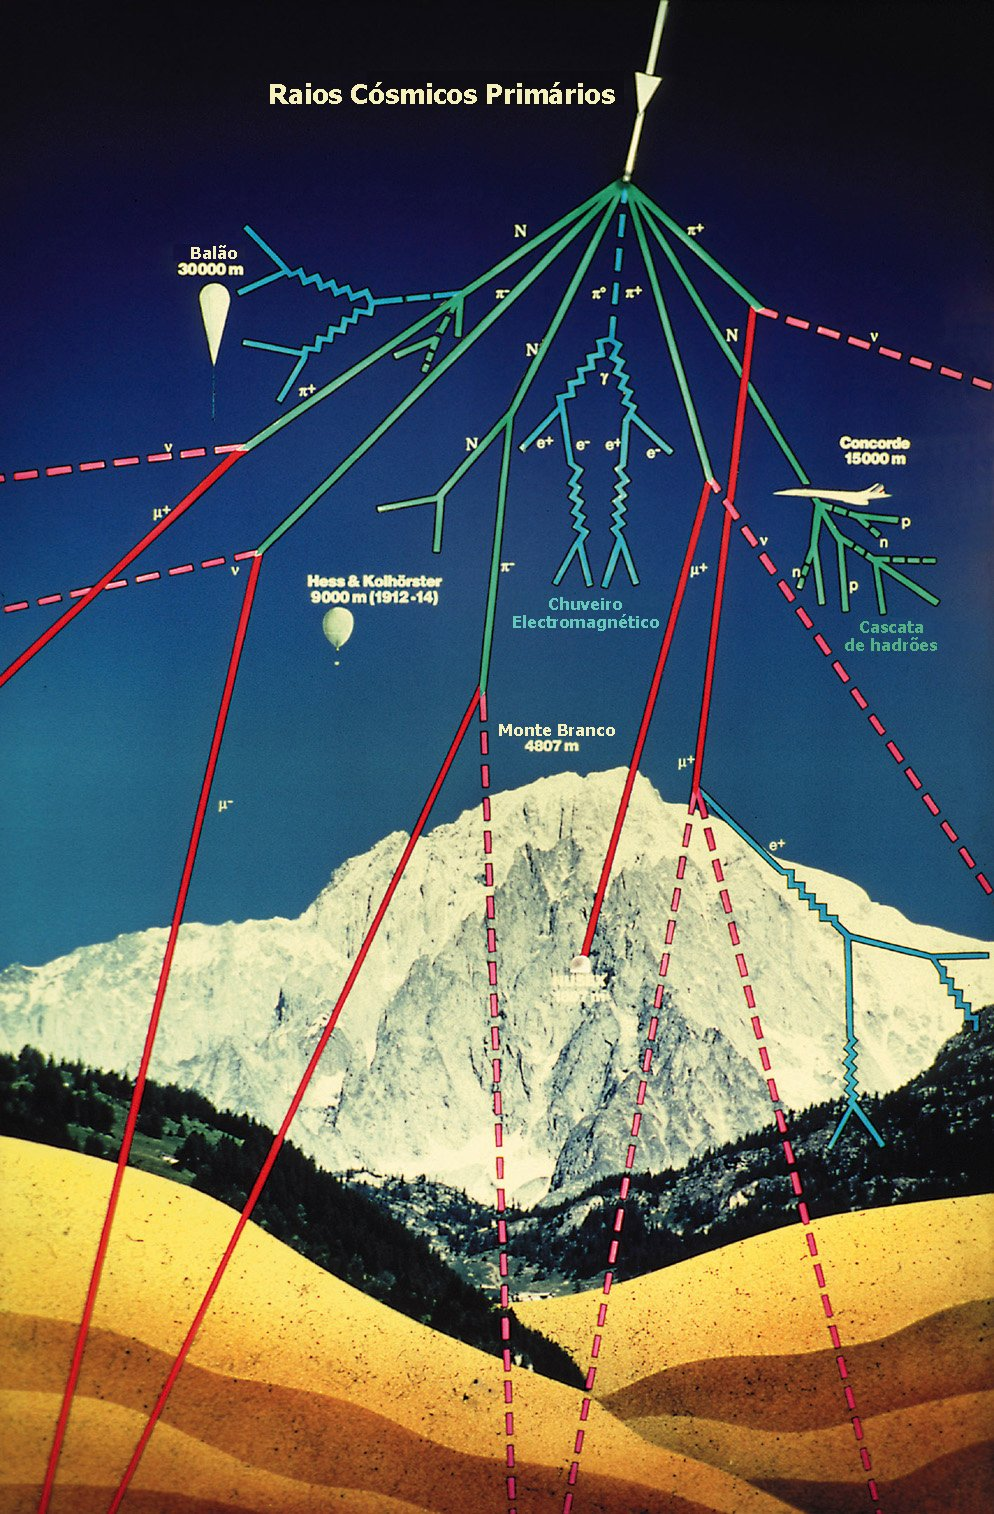
\includegraphics[width=6cm,height=8cm]{Figs/cosmics/rc_sky.png}
 \caption{Raios Cósmicos atingindo a atmosfera}
 \label{fig:rc_sky}
\end{figure}

Entre as partículas geradas, os múons possuem maior penetração na atmosfera, atingindo o detector a cem metros de profundidade e interagindo com todos os calorímetros (como visto na figura~\ref{fig:decay_chart}) dissipando pouca energia, dominantemente através da ionização dos átomos do meio (chumbo, no caso do calorímetro eletromagnético e aço no caso do hadrônico).

Raios cósmicos podem ocasionalmente depositar maiores energias devido a processos radioativos como Bremsstrahlung e produção de pares elétron-pósitron desenvolvendo chuveiros eletromagnéticos. Eles também podem produzir raios gama altamente energéticos ao interagir com os calorímetros.

No contexto da seleção de elétrons (como é o objetivo do Ringer) raios cósmicos são considerados, assim como jatos hadrônicos, ruído de fundo do experimento. Desta maneira, eventos com dados de interações de Raios Cósmicos devem ser reprovados pelos pacotes de seleção elétron/jato.

\subsubsection{Aquisição de Dados}

Os dados gerados pelo detector foram disponibilizados pela colaboração em arquivos ByteStream, que representam os dados assim como estavam na saída do sistema online de filtragem. No entanto, o formato NTuple é geralmente utilizado com o propósito de manipular os dados do experimento, uma vez que possibilita fácil e rápido acesso através do framework Root. Além disto, a ferramenta do Athena TrigRingerTools provê uma extensão do Matlab que recupera dados de NTuples e disponibiliza em formato próprio para convenientes operações com matrizes em tal ambiente.

Desta maneira, foi necessário transformar os arquivos ByteStream em NTuple mantendo a consistência dos dados. Dos possíveis métodos, o que obteve melhor resultado foi re-rodar o Athena utilizando os arquivos ByteStream como entrada e configurando o ambiente para armazenar os dados gerados em NTuples.

Durante o funcionamento do detector, o framework Data Quality Monitoring disponibiliza histogramas sumarizados de dados variados de maneira a apresentar uma estimativa qualitativa da distribuição destes dados (Figura~\ref{fig:rc_dqm}). Esta ferramenta foi importante para validar a correta recuperação dos dados em NTuples.

\begin{figure}[htbp!]
 \centering
 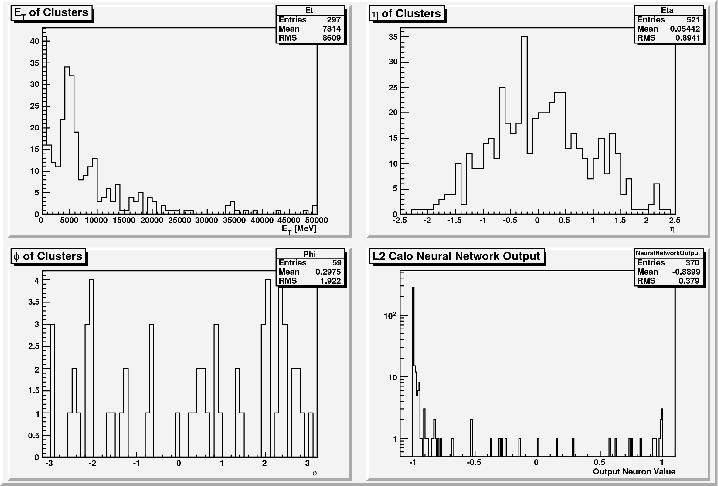
\includegraphics[width=8cm,height=6cm]{Figs/cosmics/rc_dqm.jpeg}
 \caption{Histogramas de Monitoração Online}
 \label{fig:rc_dqm}
\end{figure}

\subsubsection{Distribuições de Energia, Eta e Phi}

A distribuição para a deposição de energia de múons provenientes de raios cósmicos prevista pela teoria é uma convolução de landau com gaussiana. No entanto, é esperada também uma distribuição gaussiana em faixas de baixa energia referente ao pedestal, que por sua vez representa regiões erroneamente selecionadas pelo primeiro nível de filtragem e, desta maneira, deve estar fora do alcance do fitting de energia para raios cósmicos. O fitting realizado (Figura~\ref{fig:rc_fit}) obteve uma alta probabilidade de ser o correto para a distribuição obtida experimentalmente.

A área ao redor do MPV (most probable value - valor mais provável) da distribuição de raios cósmicos está relacionada com regiões onde a interação dos raios cósmicos foi através da ionização dos átomos do meio, justificando sua alta densidade de ocorrências e baixo valor de energia. Já a longa cauda desta distribuição está relacionada a interações mais energéticas e menos frequentes como as que ocorrem por processos radioativos.

Quanto às distribuições de eta e phi, pode-se observar que há maior densidade de eventos para valores correspondentes à região próxima ao eixo vertical central do detector ($\eta = 0$ e $\phi = \pm \frac{\pi}{2}$).

\begin{figure}[htbp!]
 \centering
 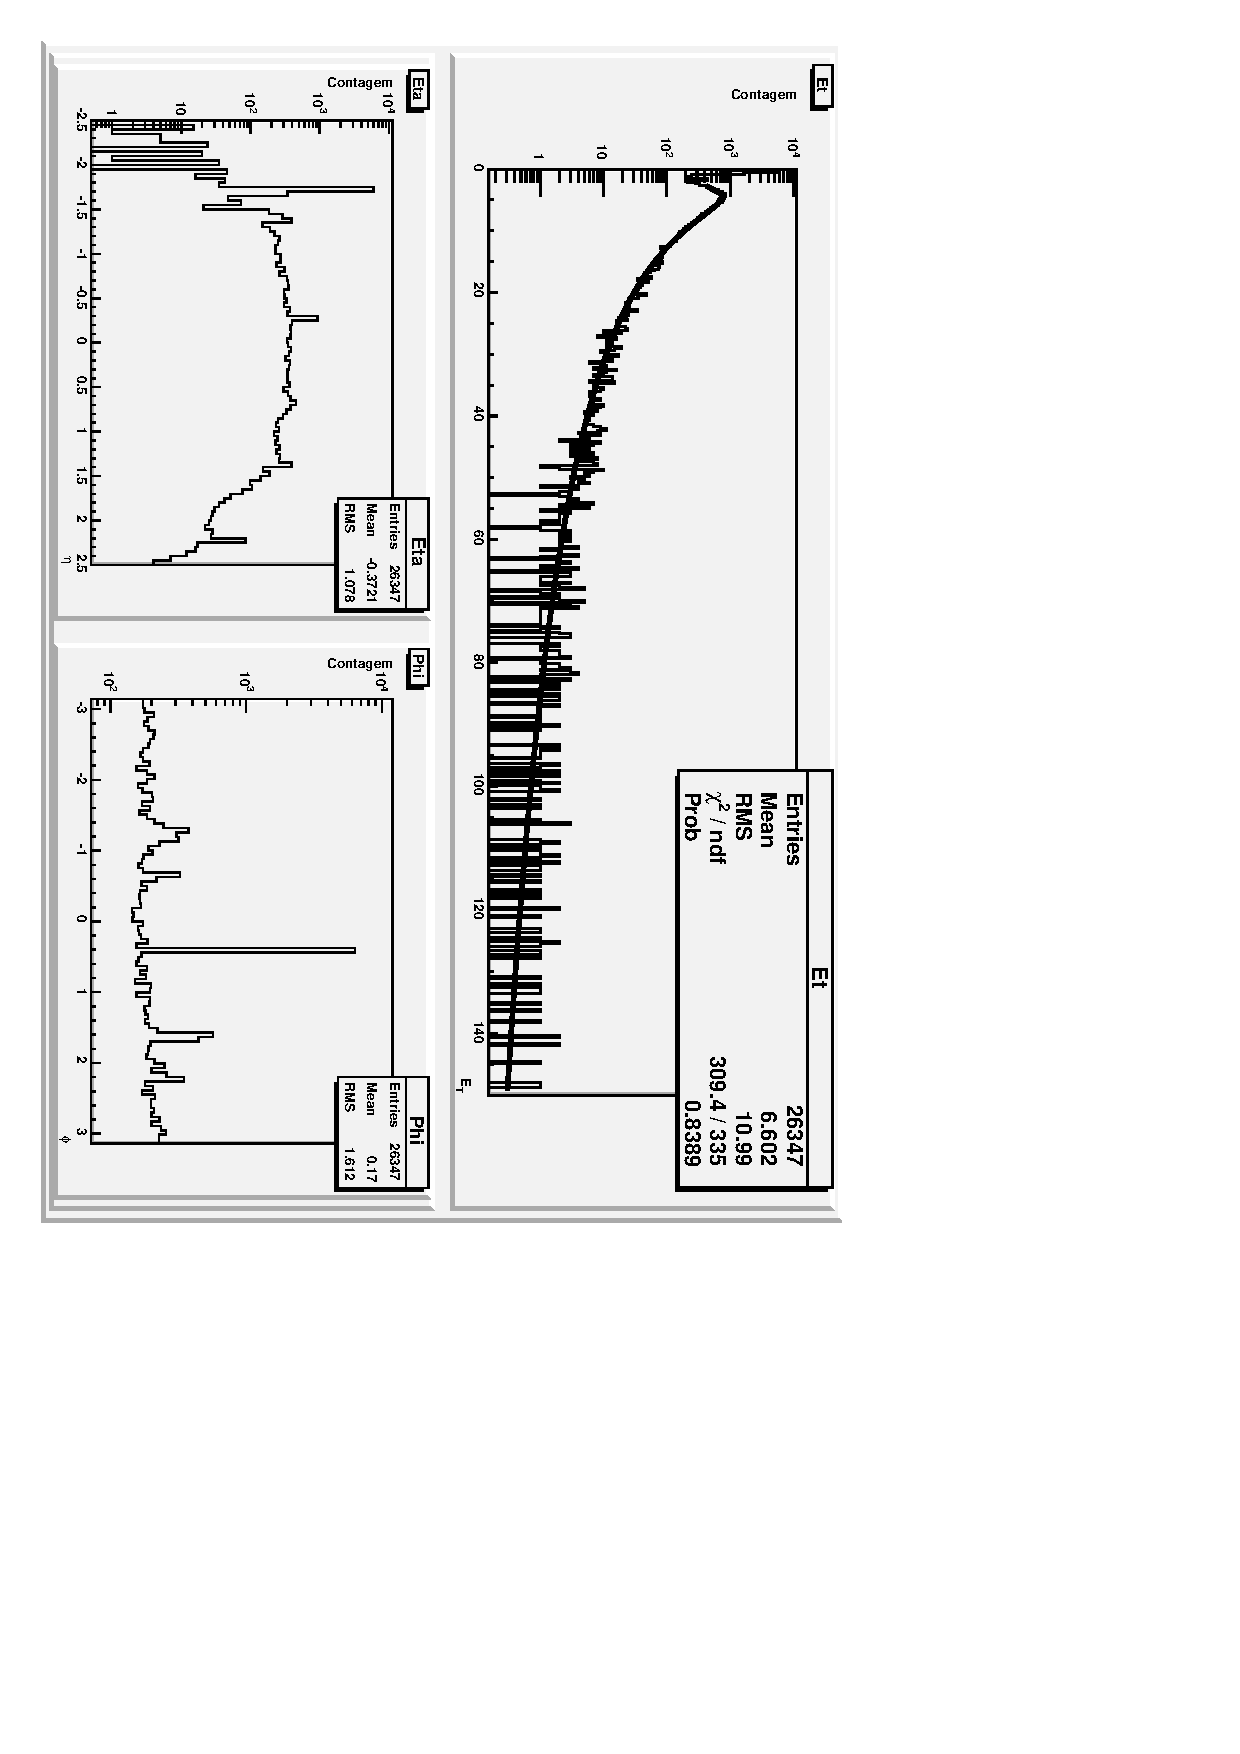
\includegraphics[width=6cm,height=10cm, angle=90]{Figs/cosmics/rc_fit.pdf}
 \caption{Distribuições de Energia, Eta e Phi para raios cósmicos}
 \label{fig:rc_fit}
\end{figure}

No entanto, alguns picos podem ser observados em ambas as distribuições. Para verificar a correlação dos picos foi então analisada a distribuição espacial $\eta \times \phi $ (Figura~\ref{fig:rc_eta_phi}) e desta maneira foi possível concluir que os picos observados separadamente nas distribuições não correspondem a faixas do detector, e sim regiões mais pontuais.

\begin{figure}[htbp!]
 \centering
 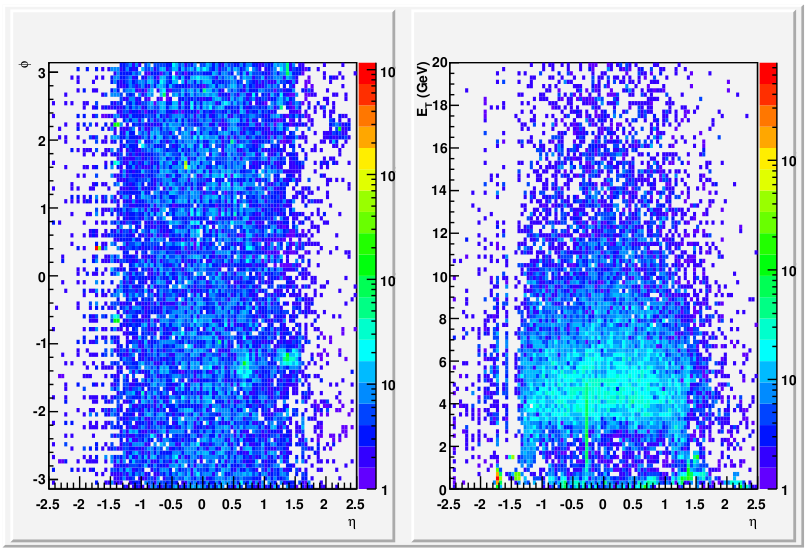
\includegraphics[width=12cm,height=8cm]{Figs/cosmics/rc_eta_phi.png}
 \caption{Distribuições espacial Eta x Phi para raios cósmicos}
 \label{fig:rc_eta_phi}
\end{figure}

\subsubsection{Células Quentes e Células Fantasmas}

Uma vez que as irregularidades encontradas não se encaixam com o previsto pela teoria, as mesmas foram investigadas. A região mais pronunciada ($\eta = -1.7, \phi = 0.4$), assim como algumas outras menos pronunciadas, apresentam alta densidade de ocorrência de valores energéticos abaixo de 1GeV. Elas são um reflexo do funcionamento inadequado da eletrônica do primeiro nível em baixas energias, uma vez que esta foi projetada para cortes em energia acima de 2 GeV. O problema se deve ao fato de que na rodada de funcionamento que gerou os dados utilizados foi utilizado um corte menor com fins de que fossem armazenados mais dados direcionados ao comissionamento do detector.

Este fenômeno pode ser chamado de "eventos fantasmas" e não deverão ser levados em consideração para análises de eficiência dos algoritmos, uma vez que não estarão presentes em rodadas de colisionamento de partículas. A figura~\ref{fig:rc_low_et} ilustra a disposição da distribuição de energia nas 4 camadas do calorímetro eletromagnético para um "evento fantasma" onde os valores são ruídos da eletrônica do primeiro nível.

\begin{figure}[htbp!]
 \centering
 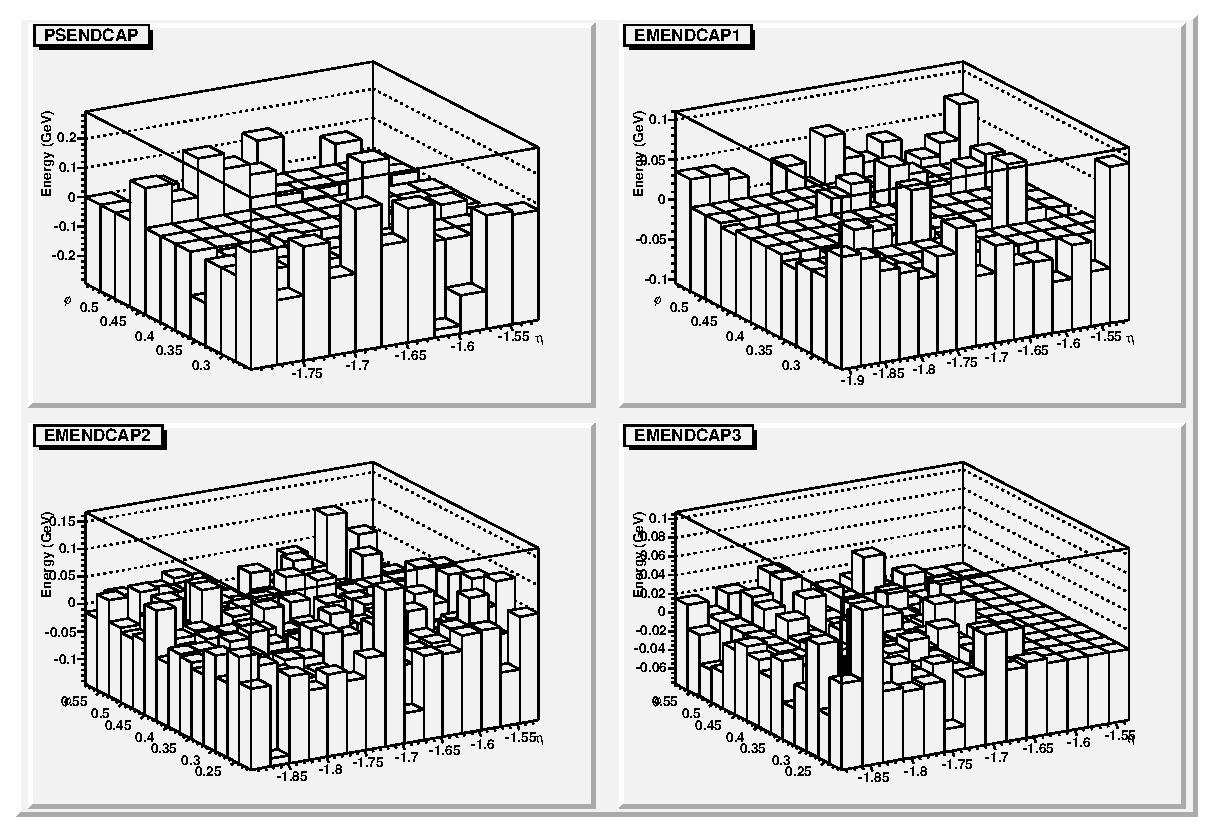
\includegraphics[width=8cm,height=6cm]{Figs/cosmics/rc_low_et.eps}
 \caption{Distribuição espacial Eta x Phi nos calorímetros eletromagnéticos para um Evento Fantasma}
 \label{fig:rc_low_et}
\end{figure}

\section{Conclusões}

Os resultados da validação apontaram que esta implementação mantém o resultado esperado tanto se comparada com a antiga propagação quanto com a propagação nativa
do Matlab. Vale ressaltar que a implementação do modelo proposto atingiu uma taxa de 99\% de detecção de elétrons para apenas 2,4\% de falso alarme, superando o algoritmo de discriminação elétron/jato vigente (T2Calo), que por sua vez atinge 96\% de detecção para 11\% de falso alarme.

O tempo de execução alcançado foi dez vezes menor do que a antiga implementação. Desta maneira, o trabalho da equipe mostra-se um potencial candidato para efetiva aplicação quando o experimento iniciar.

\section{Trabalhos Futuros}

\pagebreak

\bibliographystyle{plain}
\bibliography{ref.bib}

\pagebreak

\appendix

\section{Resumo de Trabalho Aprovado no XXX Encontro Nacional de Física de Particulas e Campos}

\begin{figure}[htbp!]
 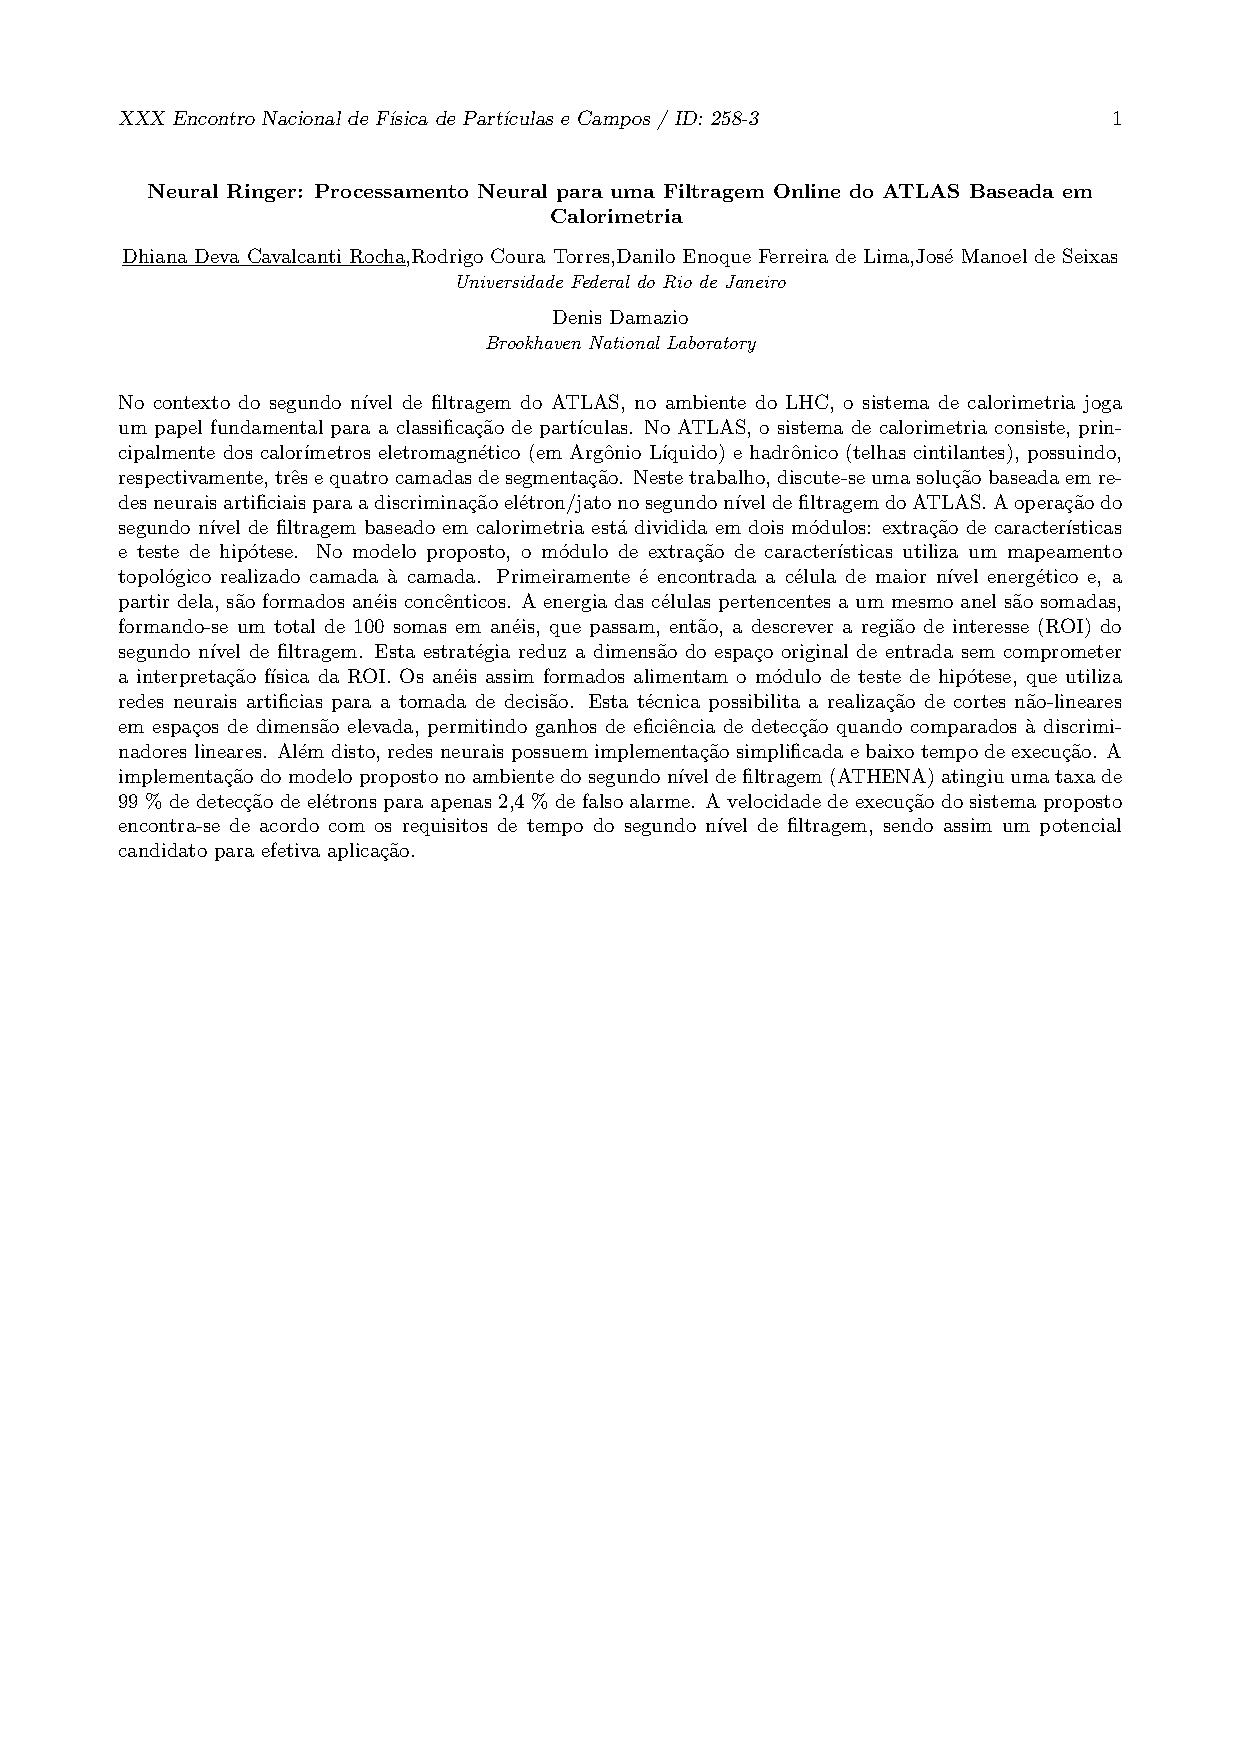
\includegraphics[scale=0.8,keepaspectratio=true,clip=true,trim=55px 300px 50px 50px]{Figs/abstracts/enfpc_xxx/R0258-3.pdf}
\end{figure}

\clearpage

\section{Resumo de Trabalho Aprovado no XXXI Encontro Nacional de Física de Particulas e Campos}

\begin{figure}[hb]
 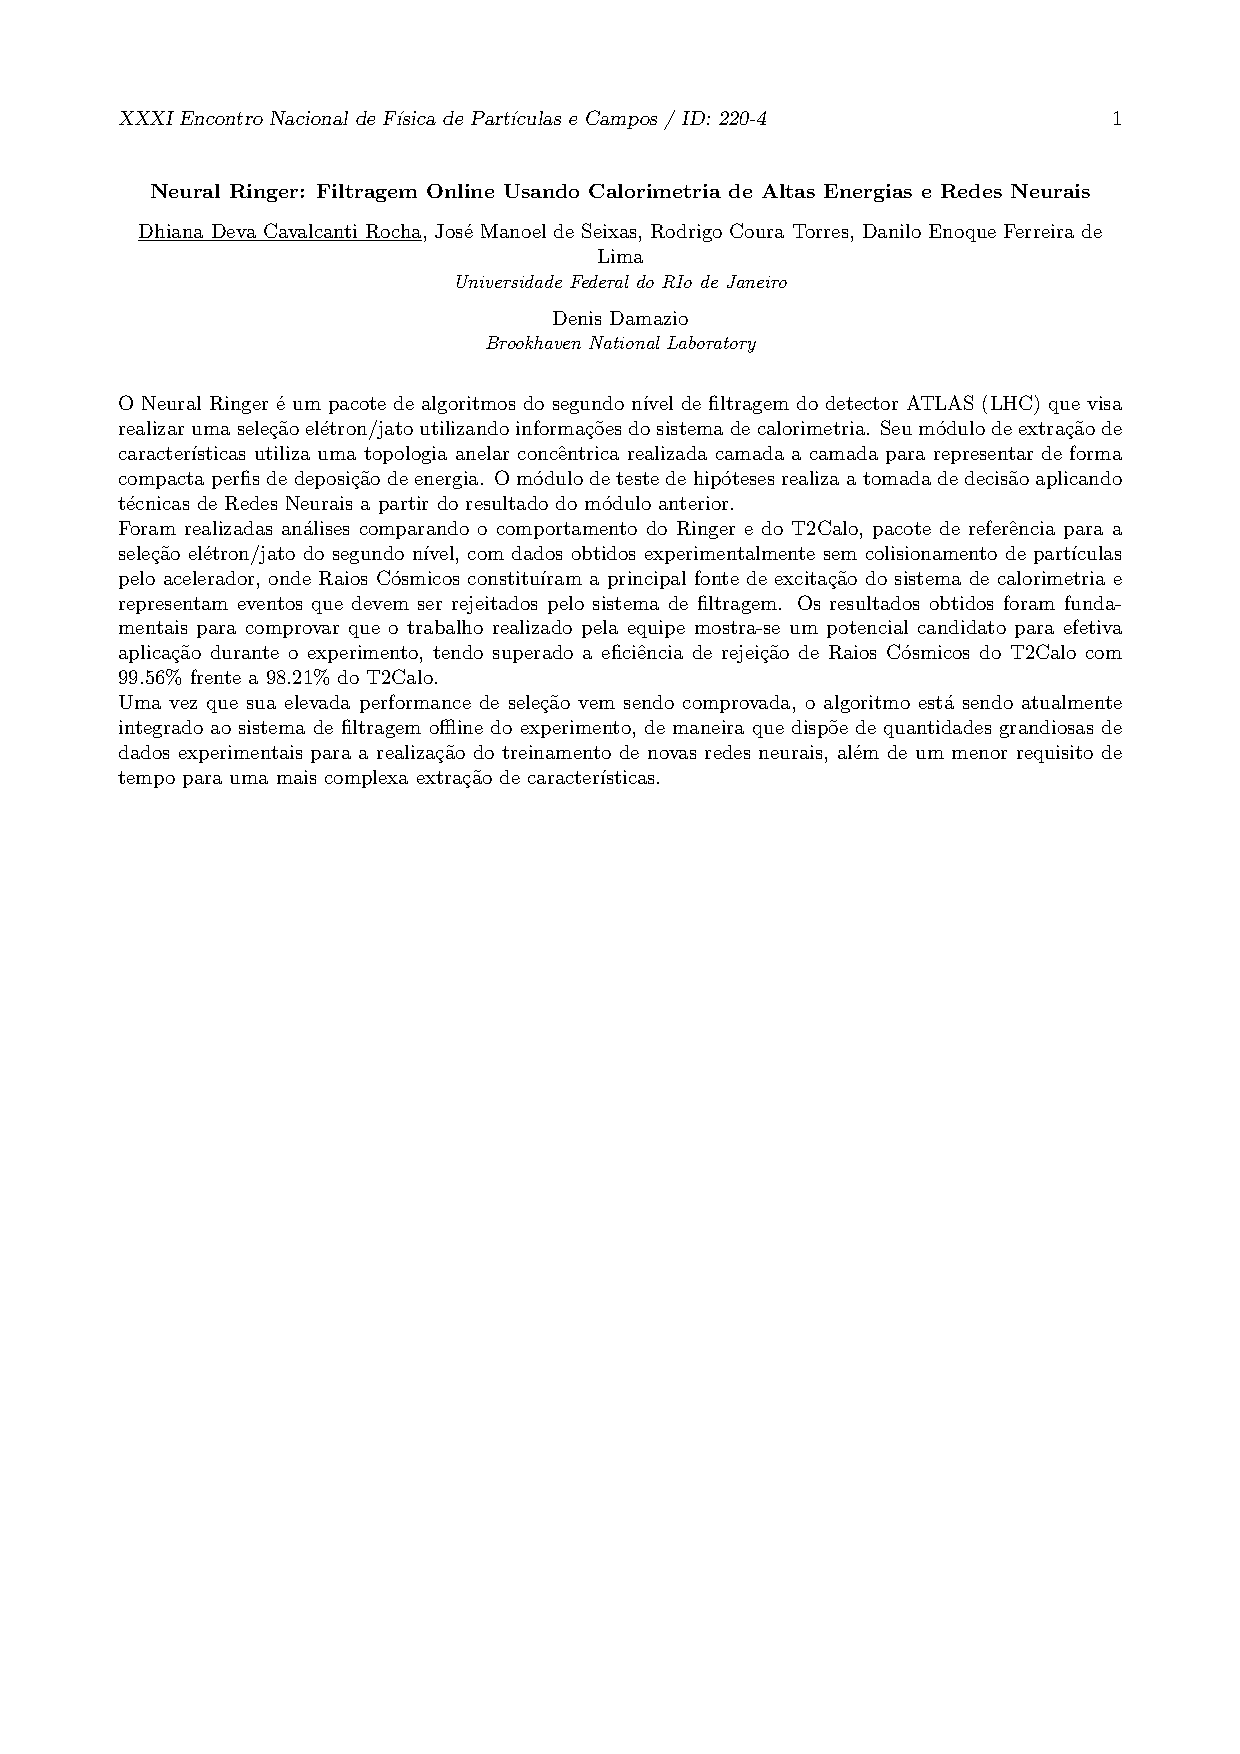
\includegraphics[scale=0.8,keepaspectratio=true,clip=true,trim=55px 300px 50px 50px]{Figs/abstracts/enfpc_xxxi/R0220-4.pdf}
\end{figure}

\clearpage

\section{Resumo de Trabalho Aprovado no XXXII Encontro Nacional de Física de Particulas e Campos}

\begin{figure}[htbp!]
 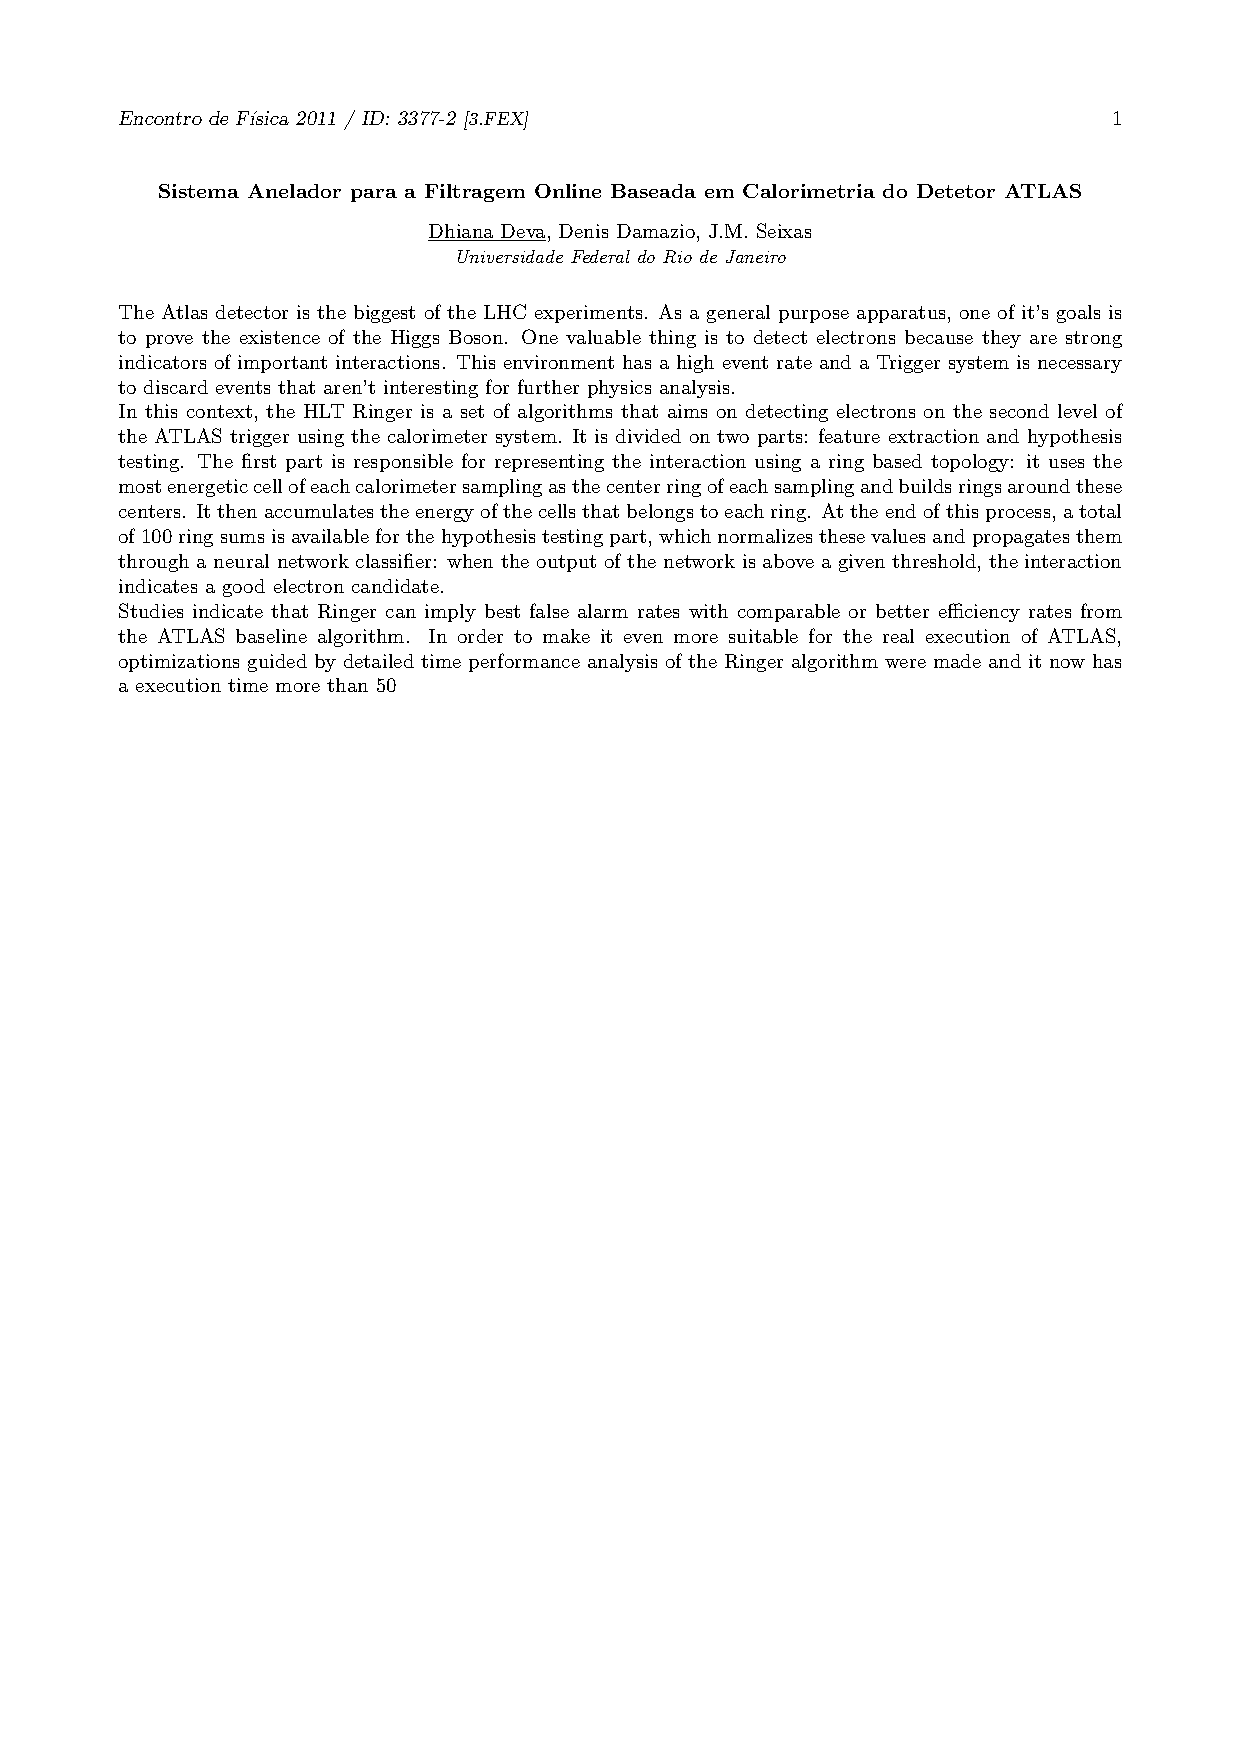
\includegraphics[scale=0.8,keepaspectratio=true,clip=true,trim=55px 300px 50px 50px]{Figs/abstracts/enfpc_xxxii/R3377-2.pdf}
\end{figure}

\clearpage

\section{Resumo de Trabalho Aprovado no 14º International Workshop on Advanced Computing and Analysis Techniques in Physics Research}

\begin{figure}[htbp!]
 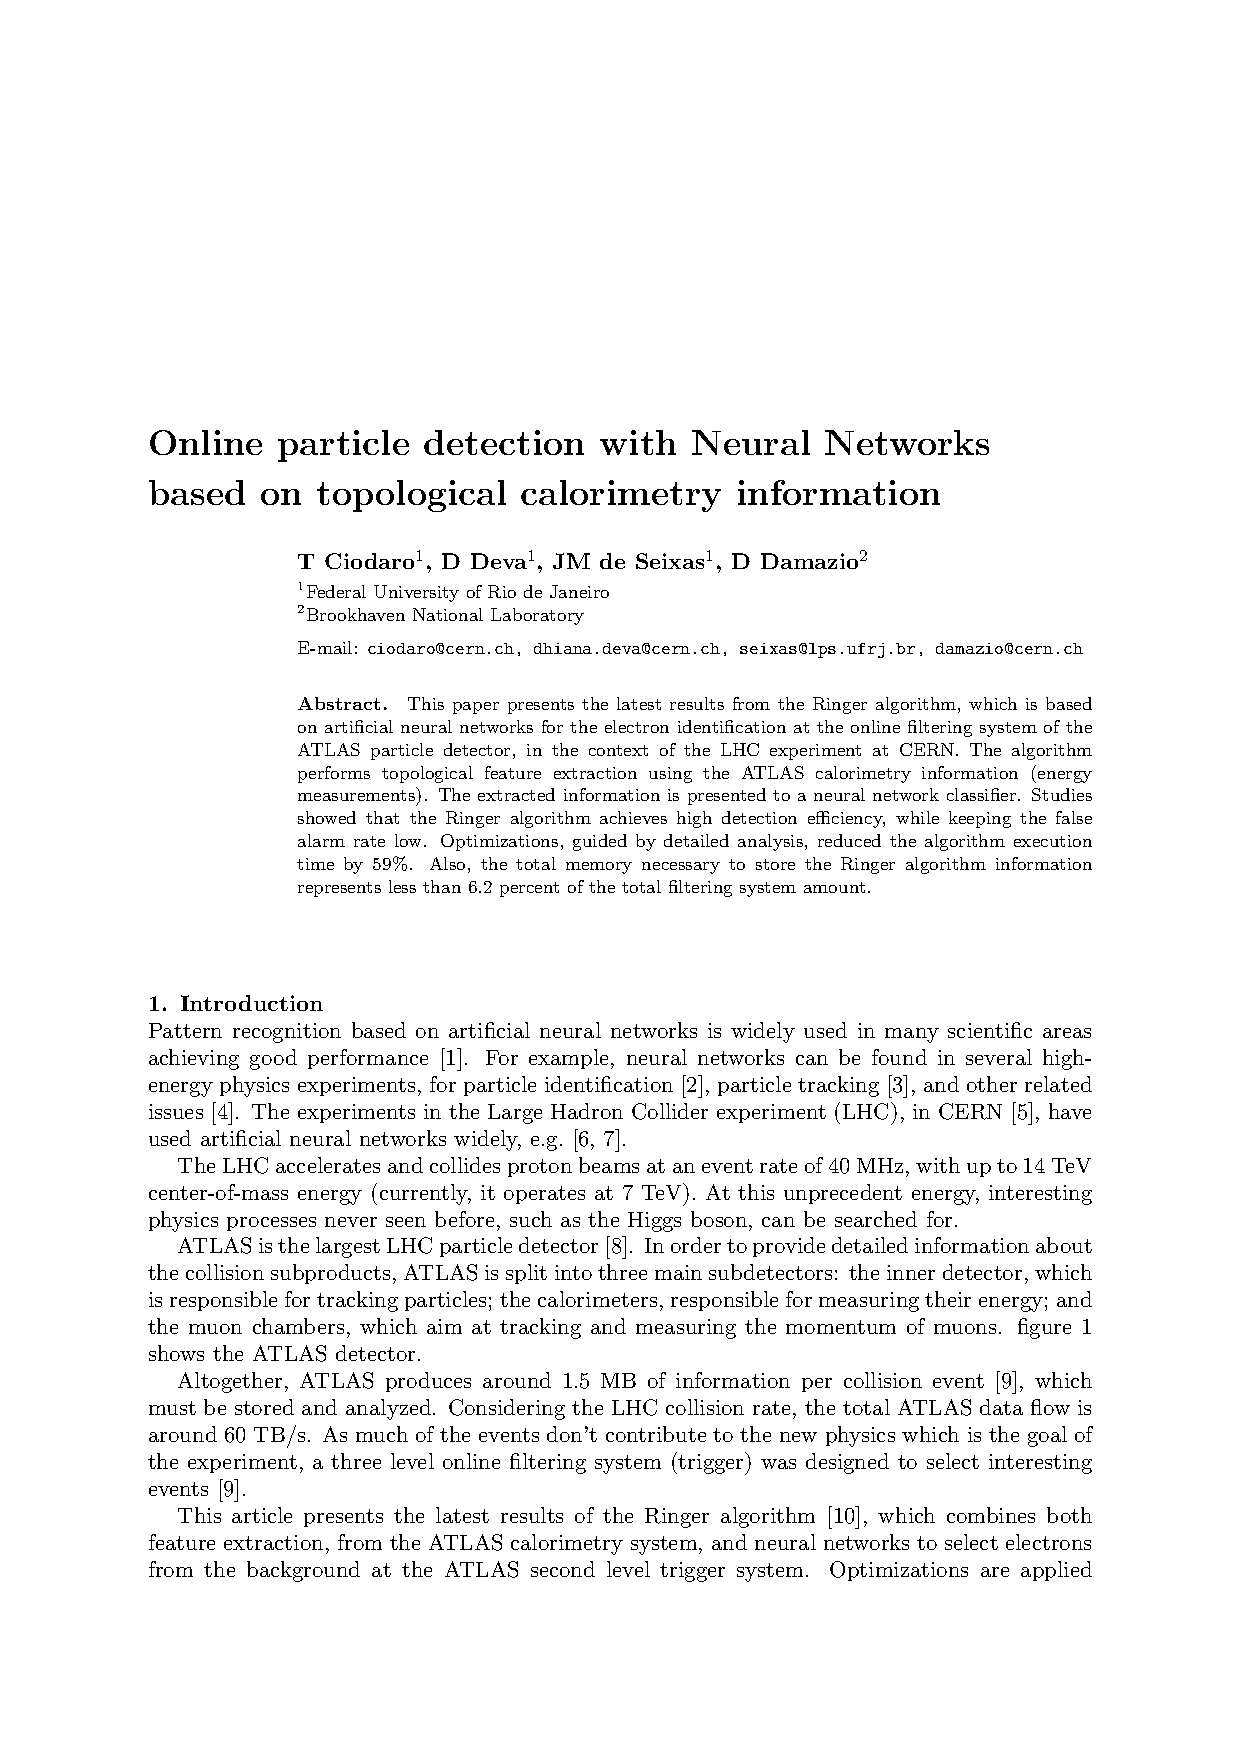
\includegraphics[scale=0.8,keepaspectratio=true,clip=true,trim=50px 400px 50px 200px]{Figs/abstracts/acat_2011/proceedings_final_30042012.pdf}
\end{figure}

\end{document}
